\documentclass[handout]{beamer}
%==============================================================
% Common Beamer Preamble for Course Lectures: Training and Scaling Language Models
%==============================================================

\usepackage[utf8]{inputenc}
\usepackage[T1]{fontenc}
\usepackage{hyperref}
\usepackage{amsmath,amssymb,xcolor,multicol,booktabs,colortbl}
\usepackage{graphicx,listings}
\renewcommand{\figurename}{Figure.}
\renewcommand{\tablename}{Table.}

% ---- TikZ Libraries ----
\usepackage{tikz}
\usetikzlibrary{positioning,arrows.meta,shapes.geometric,calc,fit,backgrounds,decorations.pathreplacing}

% ---- Presentation defaults ----
\setbeamertemplate{navigation symbols}{}
\setbeamersize{text margin left=0.55cm,text margin right=0.55cm}
\setbeamerfont{title}{size=\LARGE,series=\bfseries}
\setbeamerfont{subtitle}{size=\large}

% ---- FontAwesome fallback ----
\IfFileExists{fontawesome5.sty}{%
  \usepackage{fontawesome5}%
}{%
  \providecommand{\faMicrochip}{}%
  \providecommand{\faComments}{}%
  \providecommand{\faTools}{}%
  \providecommand{\faCheckCircle}{}%
  \providecommand{\faExclamationTriangle}{}%
  \providecommand{\faImage}{}%
  \providecommand{\faRobot}{}%
  \providecommand{\faTerminal}{}%
  \providecommand{\faBook}{}%
  \providecommand{\faRedo}{}%
  \providecommand{\faLayerGroup}{}%
  \providecommand{\faCogs}{}%
  \providecommand{\faDatabase}{}%
  \providecommand{\faHdd}{}%
  \providecommand{\faNetworkWired}{}%
}

% ---- Theme Style and Semantic Colors ----
%==============================================================
% Centralized Semantic Color Definitions for LLMs Presentation
%==============================================================

% ---- Base Template / Theme Colors (Aligned with Palette B) ----
\definecolor{themenavy}{RGB}{22,70,102}       % Palette B primary cerulean: #164666
\definecolor{themeblue}{RGB}{22,70,102}       % Primary alias
\definecolor{primarylight}{RGB}{34,92,132}    % Primary light: #225c84
\definecolor{themeteal}{RGB}{0,159,176}       % Accent cyan-teal: #009fb0
\colorlet{main_color}{themenavy}
\colorlet{accent}{themeteal}

\definecolor{accentdark}{RGB}{0,108,120}      % Deep cyan-teal for contrast text
\definecolor{accentlight}{RGB}{56,178,214}    % Slate accent cyan: #38b2d6
\definecolor{leafred}{RGB}{197,93,61}         % Terracotta red for branches/leaves

% ---- Website Panel & Border Neutrals ----
\definecolor{panelbg}{RGB}{237,245,249}       % Course-panel: #edf5f9
\definecolor{panelborder}{RGB}{204,226,238}   % Course-border: #cce2ee

% ---- Code listing style (syntax highlights) ----
\definecolor{deepblue}{RGB}{22,70,102}
\definecolor{deepred}{rgb}{0.6,0,0}
\definecolor{deepgreen}{RGB}{0,135,150}
\definecolor{halfgray}{gray}{0.55}

% ---- Semantic Theme Navy / Cerulean Shades ----
\colorlet{themebluebg}{panelbg}               % Panel #edf5f9
\colorlet{themebluecard}{main_color!8}        % Mild card background fills
\colorlet{themeblueborder}{panelborder}       % Border #cce2ee
\colorlet{themebluemid}{themeteal!60}         % Accent mid-contrast
\colorlet{themebluedraw}{main_color!80}       % Strong outline draws/strokes

% ---- Semantic Secondary Accent Teal Shades ----
\colorlet{accentdarkbg}{themeteal!10}        % Light secondary background fills
\colorlet{accentdarkdraw}{themeteal}         % Secondary outlines/strokes/text/axes

% ---- Functional Colors: Success Green ----
\definecolor{successgreen}{RGB}{55,145,55}
\colorlet{successbg}{successgreen!8}
\colorlet{successdraw}{successgreen!75}

% ---- Functional Colors: Alert Red ----
\definecolor{alertred}{RGB}{197,55,55}
\colorlet{alertbg}{alertred!8}
\colorlet{alertdraw}{alertred!75}

% ---- Functional Colors: Warning Orange ----
\definecolor{warningorange}{RGB}{220,110,30}
\colorlet{warningbg}{warningorange!10}
\colorlet{warningdraw}{warningorange!80}

% ---- Terracotta Red Shades ----
\colorlet{leafredbg}{leafred!12}
\colorlet{leafreddraw}{leafred!80}

% ---- Accent Violet (SWE-bench / observe phases) ----
\definecolor{accentviolet}{RGB}{120,70,180}
\colorlet{accentvioletbg}{accentviolet!10}
\colorlet{accentvioletdraw}{accentviolet!80}

% ---- Post-Training Axis Blue ----
\definecolor{posttrainingblue}{RGB}{40,90,165}
\colorlet{posttrainingbg}{posttrainingblue!8}
\colorlet{posttrainingdraw}{posttrainingblue!75}

% ---- Harness Component Action Green ----
\definecolor{actiongreen}{RGB}{55,145,55}
\colorlet{actiongreenbg}{actiongreen!10}
\colorlet{actiongreendraw}{actiongreen!65}

% ---- Harness Component Persist Olive ----
\definecolor{persistolive}{RGB}{120,135,40}
\colorlet{persistolivebg}{persistolive!12}
\colorlet{persistolivedraw}{persistolive!70}

% ---- Harness Component Observe Violet ----
\colorlet{observevioletbg}{accentvioletbg}
\colorlet{observevioletdraw}{accentvioletdraw}

% ---- Neutrals (Grays/Blacks) ----
\colorlet{neutralbg}{black!4}             % Very light background fills
\colorlet{neutrallight}{black!30}         % Border frames/ticks/dividers
\colorlet{neutraldark}{black!75}          % Main body text/code listing text

% ---- Beamer Block Color Overrides (Premium Terracotta Theme) ----
\setbeamercolor{block title alert}{bg=leafreddraw,fg=white}
\setbeamercolor{block body alert}{bg=leafredbg}
\setbeamercolor{alerted text}{fg=leafreddraw}

\usepackage{../common/style}
\graphicspath{{../common/figs/}{figs/}}

% ---- Code Listing Config ----
\lstset{
  basicstyle=\ttfamily\footnotesize,
  keywordstyle=\bfseries\color{deepblue},
  emphstyle=\ttfamily\color{deepred},
  stringstyle=\color{deepgreen},
  commentstyle=\color{halfgray}\itshape,
  numbers=left, numberstyle=\tiny\color{halfgray},
  backgroundcolor=\color{codebg},
  frame=l, framerule=1.5pt, rulecolor=\color{themeteal},
  xleftmargin=10pt, framexleftmargin=4pt, numbersep=6pt,
  showstringspaces=false, breaklines=true,
  aboveskip=4pt, belowskip=4pt
}

% ---- Image Placeholder Utility ----
\newcommand{\slideimage}[2][3.8cm]{%
  \begin{center}
    \begin{tikzpicture}
      \node[draw=main_color, dashed, very thick, rounded corners,
        fill=themebluebg, minimum width=0.88\linewidth, minimum height=#1,
      text width=0.80\linewidth, align=center, font=\itshape, text=accentdark]
      {\textbf{[ FIGURE / DIAGRAM ]}\\[6pt] #2};
    \end{tikzpicture}
  \end{center}
}

% ---- Concept Highlight Card Utility ----
\newcommand{\conceptcard}[3]{%
  \begin{coursebox}{#1}{#2}#3\end{coursebox}%
}

% ---- Reusable teaching-slide components ----
\newcommand{\learninggoals}[4]{%
  \begin{frame}{What should be clear by the end?}
    \begin{enumerate}
        \setlength{\itemsep}{7pt}
      \item #1
      \item #2
      \item #3
      \item #4
    \end{enumerate}
  \end{frame}
}

\newcommand{\checkpoint}[2]{%
  \begin{frame}{Checkpoint: #1}
    \begin{block}{Think, then compare}
      #2
    \end{block}
  \end{frame}
}

\newcommand{\takeaways}[4]{%
  \begin{frame}{The durable ideas}
    \begin{enumerate}
        \setlength{\itemsep}{8pt}
      \item #1
      \item #2
      \item #3
      \item #4
    \end{enumerate}
  \end{frame}
}

\newcommand{\smallsource}[1]{%
  \vfill\hfill{\tiny\color{neutraldark}Source: #1}
}

% ---- Logo on content frames ----
\newif\ifplacelogo
\placelogotrue
\logo{\ifplacelogo
  \raisebox{-0.3ex}{
\includegraphics[height=0.4cm]{IMT_Atlantique_logo.png}}%
\fi}

\makeatletter
\define@key{beamerframe}{nologo}[true]{%
  \placelogofalse
}
\makeatother

% Fix Beamer bold font warning: substitute undefined T1/cmss/b/n with T1/cmss/bx/n
\DeclareFontShape{T1}{cmss}{b}{n}{<->ssub * cmss/bx/n}{}

% Default Author & Institute metadata
\author[Jonathan Lys]{Jonathan Lys}
\institute[IMT Atlantique]{IMT Atlantique}

% ---- Front Page / Title Slide Macro ----
% Displays Title + IMT Atlantique logo and Brain logo
\newcommand{\makelecturetitle}[1][Training and Scaling Language Models: From First Principles to Efficient Serving]{%
  \placelogofalse
  {
    \setbeamertemplate{footline}{}
    \settitletagline{#1}
    \settitlelogos{%
      \raisebox{-0.5\height}{
\includegraphics[height=1.15cm]{IMT_Atlantique_logo.png}}%
      \hspace{1.2em}%
      \raisebox{-0.5\height}{\includegraphics[height=1.15cm]{brain.pdf}}}
    \begin{frame}[plain]
      \titlepage
    \end{frame}
  }
  \placelogotrue
}

% Section TOC Frame
\AtBeginSection[]{\coursesectiondivider}


\title[TLM -- Session 05]{Session 5: Data Selection through FineWeb\\[4pt]
\normalsize\itshape Turning ``Quality'' into a Testable Pipeline}
\date{\today}

\begin{document}
\makelecturetitle

\begin{frame}{Lecture map}
  \tableofcontents
  \vfill
  \begin{block}{Guiding question}
    How can a filtering decision be evaluated before and after spending compute on pretraining?
  \end{block}
\end{frame}

\learninggoals
  {Reconstruct the stages and design logic of the FineWeb pipeline.}
  {Distinguish extraction, filtering, deduplication, and learned selection.}
  {Explain why plausible heuristics still require ablations.}
  {Design a fair token-matched comparison with contamination controls.}

\section{Web data becomes a training distribution}

\begin{frame}{Data quality is an operational claim}
  \begin{block}{A useful definition}
    Corpus $A$ is better than corpus $B$ for a stated goal if training under the same compute, token, model, and evaluation contract yields stronger evidence on that goal.
  \end{block}
  \begin{alertblock}{What ``cleaner'' does not establish}
    Human preference, lower toxicity, fewer duplicates, and benchmark performance are related but different objectives. Name which one the selector targets.
  \end{alertblock}
  \vfill
  \centering Selection changes the model's empirical world. It is part of the model design.
\end{frame}

\begin{frame}{FineWeb turns Common Crawl into a staged experiment}
  \centering
  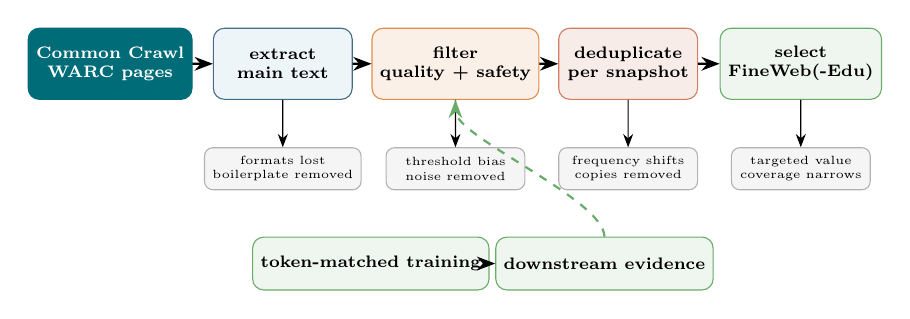
\begin{tikzpicture}[x=1cm,y=1cm,scale=.86,transform shape,
    stage/.style={draw=themebluedraw,fill=themebluebg,rounded corners=4pt,minimum width=2.05cm,minimum height=1.05cm,align=center,font=\scriptsize\bfseries},
    consequence/.style={draw=neutrallight,fill=neutralbg,rounded corners=3pt,minimum width=2.05cm,minimum height=.62cm,align=center,font=\tiny},
    eval/.style={draw=successdraw,fill=successbg,rounded corners=4pt,minimum width=2.8cm,minimum height=.78cm,align=center,font=\scriptsize\bfseries}]
    \node[stage,fill=accentdark,draw=accentdark,text=white] (w) at (0,2.7) {Common Crawl\\WARC pages};
    \node[stage] (e) at (2.55,2.7) {extract\\main text};
    \node[stage,fill=warningbg,draw=warningdraw] (f) at (5.10,2.7) {filter\\quality + safety};
    \node[stage,fill=leafredbg,draw=leafreddraw] (d) at (7.65,2.7) {deduplicate\\per snapshot};
    \node[stage,fill=successbg,draw=successdraw] (q) at (10.20,2.7) {select\\FineWeb(-Edu)};
    \foreach \a/\b in {w/e,e/f,f/d,d/q}{\draw[-{Stealth},thick] (\a)--(\b);}
    \node[consequence] (ce) at (2.55,1.15) {formats lost\\boilerplate removed};
    \node[consequence] (cf) at (5.10,1.15) {threshold bias\\noise removed};
    \node[consequence] (cd) at (7.65,1.15) {frequency shifts\\copies removed};
    \node[consequence] (cq) at (10.20,1.15) {targeted value\\coverage narrows};
    \foreach \a/\b in {e/ce,f/cf,d/cd,q/cq}{\draw[-{Stealth},thin] (\a)--(\b);}
    \node[eval] (train) at (3.85,-.25) {token-matched training};
    \node[eval] (measure) at (7.30,-.25) {downstream evidence};
    \draw[-{Stealth},thick] (train)--(measure);
    \draw[-{Stealth},thick,dashed,successdraw] (measure.north) .. controls +(0,.55) and +(0,-.55) .. (f.south);
  \end{tikzpicture}
  \par\vspace{2pt}
  \footnotesize The recipe is validated by the model it produces, not by cleanliness alone.\par
  \smallsource{Penedo et al., The FineWeb Datasets and Hugging Face FineWeb blog}
\end{frame}

\begin{frame}{Extraction is already a selection function}
  HTML contains navigation, cookie dialogs, comments, ads, hidden text, and main prose.
  \vspace{5pt}
  \begin{columns}[t]
    \begin{column}{0.47\linewidth}
      \begin{block}{High recall extractor}
        Keeps more useful prose but also more boilerplate and malformed text.
      \end{block}
    \end{column}
    \begin{column}{0.47\linewidth}
      \begin{alertblock}{High precision extractor}
        Produces cleaner documents but may erase code, lists, tables, and minority formats.
      \end{alertblock}
    \end{column}
  \end{columns}
  \vfill
  Inspect raw HTML, extracted text, and rejection reason together. Otherwise, the selection mechanism is invisible.
\end{frame}

\begin{frame}{Base filters encode hypotheses about usefulness}
  \small
  \begin{tabular}{@{}>{\raggedright\arraybackslash}p{.22\linewidth}>{\raggedright\arraybackslash}p{.34\linewidth}>{\raggedright\arraybackslash}p{.34\linewidth}@{}}
    \toprule
    Signal & Hypothesis & Risk \\
    \midrule
    character or word length & fragments teach little & removes concise answers \\
    repeated lines or n-grams & boilerplate is low value & removes poetry and code \\
    symbol ratios & noise has unusual composition & harms math-heavy pages \\
    language score & target language dominates & harms multilingual content \\
    blocked URLs or domains & known sources are undesirable & domain bias \\
    \bottomrule
  \end{tabular}
  \vfill
  \begin{block}{Every threshold is an ablation candidate}
    Count removals, sample both sides of the threshold, and compare downstream behavior.
  \end{block}
\end{frame}

\section{Deduplication and learned selection}

\begin{frame}{Duplicate is not one relation}
  \begin{columns}[t]
    \begin{column}{0.31\linewidth}
      \begin{block}{Exact}
        identical normalized text or hash
      \end{block}
    \end{column}
    \begin{column}{0.31\linewidth}
      \begin{block}{Near duplicate}
        high overlap of word or character shingles
      \end{block}
    \end{column}
    \begin{column}{0.31\linewidth}
      \begin{block}{Semantic}
        same information with different surface form
      \end{block}
    \end{column}
  \end{columns}
  \vfill
  \begin{alertblock}{Design choices}
    Normalization, shingle size, similarity threshold, representative choice, and deduplication scope all change what survives.
  \end{alertblock}
\end{frame}

\begin{frame}{MinHash estimates Jaccard similarity cheaply}
  For shingle sets $A$ and $B$:
  \[
    J(A,B)=\frac{|A\cap B|}{|A\cup B|}
  \]
  A random min-wise hash satisfies:
  \[
    \Pr[\min h(A)=\min h(B)]=J(A,B)
  \]
  Repeating hashes creates a signature. Locality-sensitive buckets generate candidate pairs without comparing every document pair.
  \begin{block}{Interpretation}
    MinHash approximates set overlap. It is not a semantic similarity oracle.
  \end{block}
\end{frame}

\begin{frame}{FineWeb made deduplication scope an empirical question}
  \begin{columns}[c]
    \begin{column}{0.49\linewidth}
      \begin{block}{Global deduplication}
        Removes copies across all crawl snapshots. It maximizes novelty but can strongly alter the time and source distribution.
      \end{block}
    \end{column}
    \begin{column}{0.47\linewidth}
      \begin{block}{Per-snapshot deduplication}
        Removes repeated pages inside a crawl while preserving recurrence across time.
      \end{block}
    \end{column}
  \end{columns}
  \begin{alertblock}{Lesson from the reported ablation}
    More aggressive deduplication did not automatically yield better downstream models. A sensible mechanism still needs token-matched training evidence.
  \end{alertblock}
\end{frame}

\begin{frame}{FineWeb-Edu learns a narrower notion of value}
  \begin{enumerate}
    \setlength{\itemsep}{7pt}
    \item An LLM scores pages for educational usefulness.
    \item A smaller classifier learns to imitate those labels at corpus scale.
    \item Thresholds trade retained volume against the targeted quality signal.
  \end{enumerate}
  \begin{columns}[t]
    \begin{column}{0.47\linewidth}
      \begin{block}{Potential benefit}
        Scalable selection for explanatory, knowledge-rich text.
      \end{block}
    \end{column}
    \begin{column}{0.47\linewidth}
      \begin{alertblock}{Potential bias}
        The teacher rubric and classifier can narrow style, language, and topic coverage.
      \end{alertblock}
    \end{column}
  \end{columns}
\end{frame}

\checkpoint{selector disagreement}
  {A heuristic rejects a document that the educational classifier scores highly. What evidence would help decide whether the conflict reveals noise, a blind spot, or a genuinely different objective?}

\section{A fair data ablation}

\begin{frame}{Match the experiment, not only the dataset size}
  Keep constant:
  \begin{itemize}
    \setlength{\itemsep}{6pt}
    \item model initialization and architecture
    \item tokenizer and sequence length
    \item tokens seen, optimizer updates, and learning-rate schedule
    \item evaluation token budget and benchmark harness
    \item hardware and throughput measurement method
  \end{itemize}
  \begin{alertblock}{Replacement policy matters}
    If filtering removes data, decide whether to train on fewer unique tokens, resample survivors, or draw more raw data. These test different claims.
  \end{alertblock}
\end{frame}

\begin{frame}{Evaluate the selector before training}
  \begin{columns}[t]
    \begin{column}{0.47\linewidth}
      \begin{block}{Retention profile}
        tokens and documents kept\\language and domain shifts\\length and source distributions
      \end{block}
    \end{column}
    \begin{column}{0.47\linewidth}
      \begin{block}{Error analysis}
        sample accepted and rejected pages\\label false positives and false negatives\\inspect threshold neighborhoods
      \end{block}
    \end{column}
  \end{columns}
  \vfill
  \centering A selector can be precise on average and still erase a small but important domain.
\end{frame}

\begin{frame}{Evaluate the trained models at equal budgets}
  \begin{enumerate}
    \setlength{\itemsep}{7pt}
    \item Compare validation loss on declared distributions.
    \item Measure downstream tasks relevant to the selection objective.
    \item Report training throughput and tokens required to reach a target loss.
    \item Repeat enough seeds to separate a trend from run noise.
  \end{enumerate}
  \begin{block}{A strong claim}
    ``At equal tokens and architecture, filter $F$ reaches the same validation loss in fewer updates on distribution $D$.''
  \end{block}
\end{frame}

\begin{frame}{Contamination can imitate data quality}
  \begin{itemize}
    \setlength{\itemsep}{8pt}
    \item Search for benchmark examples and close variants before training.
    \item Split related pages and document versions together.
    \item Record the order of deduplication, split assignment, and benchmark filtering.
    \item Report contaminated and cleaned evaluations separately when needed.
  \end{itemize}
  \begin{alertblock}{Core warning}
    Higher benchmark accuracy is not evidence of better generalization if evaluation text leaked into pretraining.
  \end{alertblock}
\end{frame}

\checkpoint{pre-register the comparison}
  {Write one target claim, the baseline corpus, the selected corpus, the token replacement policy, two pre-training diagnostics, and two post-training metrics.}

\takeaways
  {Extraction and filtering define the training distribution before tokenization begins.}
  {Deduplication has a similarity definition, threshold, representative rule, and scope.}
  {FineWeb shows that plausible pipeline choices need controlled training ablations.}
  {Contamination controls and token-matched budgets are prerequisites for quality claims.}

\end{document}
